%%%%%%%%%%%%%%%%%%%%%%%%%%%%%%%%%%%%%%%%%
% The Legrand Orange Book
% LaTeX Template
% Version 3.1 (February 18, 2022)
%
% This template originates from:
% https://www.LaTeXTemplates.com
%
% Authors:
% Vel (vel@latextemplates.com)
% Mathias Legrand (legrand.mathias@gmail.com)
%
% License:
% CC BY-NC-SA 4.0 (https://creativecommons.org/licenses/by-nc-sa/4.0/)
%
% Compiling this template:
% This template uses biber for its bibliography and makeindex for its index.
% When you first open the template, compile it from the command line with the 
% commands below to make sure your LaTeX distribution is configured correctly:
%
% 1) pdflatex main
% 2) makeindex main.idx -s indexstyle.ist
% 3) biber main
% 4) pdflatex main x 2
%
% After this, when you wish to update the bibliography/index use the appropriate
% command above and make sure to compile with pdflatex several times 
% afterwards to propagate your changes to the document.
%
%%%%%%%%%%%%%%%%%%%%%%%%%%%%%%%%%%%%%%%%%

%----------------------------------------------------------------------------------------
%	PACKAGES AND OTHER DOCUMENT CONFIGURATIONS
%----------------------------------------------------------------------------------------

\documentclass[
	11pt, % Default font size, select one of 10pt, 11pt or 12pt
	fleqn, % Left align equations
	a4paper, % Paper size, use either 'a4paper' for A4 size or 'letterpaper' for US letter size
	%oneside, % Uncomment for oneside mode, this doesn't start new chapters and parts on odd pages (adding an empty page if required), this mode is more suitable if the book is to be read on a screen instead of printed
]{LegrandOrangeBook}

\usepackage{bm}
\usepackage{array}

% Book information for PDF metadata, remove/comment this block if not required 
\hypersetup{
	pdftitle={Title}, % Title field
	pdfauthor={Author}, % Author field
	pdfsubject={Subject}, % Subject field
	pdfkeywords={Keyword1, Keyword2, ...}, % Keywords
	pdfcreator={LaTeX}, % Content creator field
}

\addbibresource{sample.bib} % Bibliography file

\definecolor{ocre}{RGB}{243, 102, 25} % Define the color used for highlighting throughout the book

\chapterimage{orange1.jpg} % Chapter heading image
\chapterspaceabove{6.5cm} % Default whitespace from the top of the page to the chapter title on chapter pages
\chapterspacebelow{6.75cm} % Default amount of vertical whitespace from the top margin to the start of the text on chapter pages

%----------------------------------------------------------------------------------------

\begin{document}

%----------------------------------------------------------------------------------------
%	TITLE PAGE
%----------------------------------------------------------------------------------------

\titlepage % Output the title page
	{
\includegraphics[width=\paperwidth]{background.pdf}} % Code to output the background image, which should be the same dimensions as the paper to fill the page entirely; leave empty for no background image
	{ % Title(s) and author(s)
		\centering\sffamily % Font styling
		{\Huge\bfseries Poromecânica\par} % Book title
		\vspace{16pt} % Vertical whitespace
		{\LARGE \par} % Subtitle
		\vspace{24pt} % Vertical whitespace
		{\huge\bfseries Olivier Coussy\par} % Author name
	}

%----------------------------------------------------------------------------------------
%	COPYRIGHT PAGE
%----------------------------------------------------------------------------------------

\thispagestyle{empty} % Suppress headers and footers on this page

~\vfill % Push the text down to the bottom of the page

\noindent Copyright \copyright\ 2022 Goro Akechi\\ % Copyright notice

\noindent \textsc{Published by Publisher}\\ % Publisher

\noindent \textsc{\href{https://www.latextemplates.com/template/legrand-orange-book}{book-website.com}}\\ % URL

\noindent Licensed under the Creative Commons Attribution-NonCommercial 4.0 License (the ``License''). You may not use this file except in compliance with the License. You may obtain a copy of the License at \url{https://creativecommons.org/licenses/by-nc-sa/4.0}. Unless required by applicable law or agreed to in writing, software distributed under the License is distributed on an \textsc{``as is'' basis, without warranties or conditions of any kind}, either express or implied. See the License for the specific language governing permissions and limitations under the License.\\ % License information, replace this with your own license (if any)

\noindent \textit{First printing, March 2022} % Printing/edition date

%----------------------------------------------------------------------------------------
%	TABLE OF CONTENTS
%----------------------------------------------------------------------------------------

\pagestyle{empty} % Disable headers and footers for the following pages

\tableofcontents % Output the table of contents

\listoffigures % Output the list of figures, comment or remove this command if not required

\listoftables % Output the list of tables, comment or remove this command if not required

\pagestyle{fancy} % Enable default headers and footers again

\cleardoublepage % Start the following content on a new page

%----------------------------------------------------------------------------------------
%	PART
%----------------------------------------------------------------------------------------

\part{Part One Title}

%----------------------------------------------------------------------------------------
%	SECTIONING EXAMPLES CHAPTER
%----------------------------------------------------------------------------------------

\chapterimage{orange2.jpg} % Chapter heading image
\chapterspaceabove{6.75cm} % Whitespace from the top of the page to the chapter title on chapter pages
\chapterspacebelow{7.25cm} % Amount of vertical whitespace from the top margin to the start of the text on chapter pages

%------------------------------------------------

\chapter{Capítulo 1 - Deformação e Cinemática. Balanço de massa}\index{Sectioning}

O objetivo deste capítulo é descrever a deformação e a cinemática de um meio poroso formado por um esqueleto deformável e um fluído saturando o espaço poroso. A ideia subjacente consiste em abordar o meio poroso como a sobreposição de dois contínuos, o esqueleto contínuo e o fluído contínuo. A descrição da deformação e da cinemática de cada contínuo em separado não difere forma de alguma daquela de um meio contínuo monofásico. Mesmo assim, a deformação do esqueleto \footnote{N.T: como será visto, o \textbf{esqueleto} é o espaço ocupado pela matriz e os vazios conectados. Sendo a \textbf{matriz} o espaço ocupado pelo sólido com sua porosidade oclusa.} é a única que eventualmente pode ser realmente observada e portanto é a discutida na sequência.

As leis da física que governam a evolução de um contínuo poroso envolve a taxa temporal das quantidades físicas ligadas ao esqueleto ou ao fluído, qualquer que sejam seus movimentos distintos posterior. Por conseguinte a derivada particular é portanto introduzida, permitindo a nós seguir separadamente o movimento do esqueleto e do fluído. Uma primeira ilustração do seu uso é dada no final desse capítulo expressando o balanço de massa para os dois contínuos sobrepostos.

\section{Deformação e Cinemática. Balanço de Massa}\index{Sectioning!Sections}


\subsection{O meio poroso e a abordagem contínua}\index{Sectioning!Subsections}

Um \textbf{meio poroso saturado} é composto de uma matriz e um espaço poroso, sendo este último preenchido por um fluído. O \textbf{espaço poroso conectado} é o espaço através do qual o fluido realmente flui e cujos dois pontos podem ser unidos por um caminho inteiramente dentro dele, de modo que a fase fluída permanece contínua lá. A \textbf{matriz} é composta por uma parte sólida e uma possível porosidade oclusa saturada ou não, mas através da qual não ocorre infiltração. A \textbf{porosidade conectada} é a razão entre o volume do espaço poroso conectado e o volume total. No que segue, o termo "porosidade", usado sem maiores especificações, refere-se a toda a porosidade conectada.

\subsection{Parciculas do Esqueleto e do Fluído. Hipóteses da Continuidade}\index{Sectioning!Subsections}

Um meio poroso pode ser tratado como a sobreposição de dois contínuos, o esqueleto contínuo e o fluído contínuo. Portanto, como ilustrado na \autoref{fig:fig1-1.pdf}, qualquer volume infinitesimal pode ser tratado como a sobreposição de duas partículas materiais. A primeira é a \textbf{partícula de esqueleto} formada da matriz e do espaço poroso conectado esvaziado de fluído. A segunda é a \textbf{partícula de fluído} formada a partir do fluído que satura o espaço poroso conectado e do restante do espaço sem a matriz.

\begin{figure}[H] % Use [H] to suppress floating and place the figure/table exactly where it is specified in the text
	\centering % Horizontally center the figure on the page
	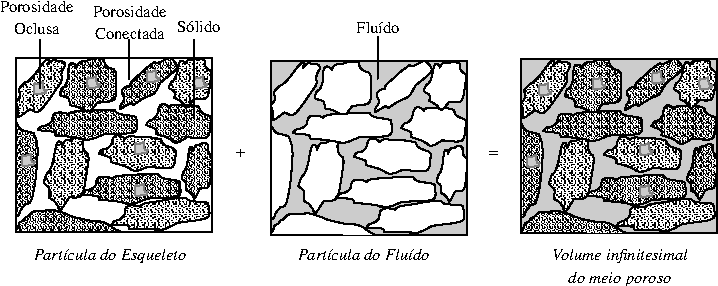
\includegraphics[scale = 1.1]{fig1-1.pdf} % Include the figure image
	\caption{O meio poroso como a superposição de dois meios contínuos: a partícula do esqueleto e uma partícula do fluído coincidentes no mesmo volume geométrico infinitesimal}
	\label{fig:fig1-1.pdf} % Unique label used for referencing the figure in-text
\end{figure}

Uma descrição contínua de um meio, que é heterogêneo na escala microscópica, requer a escolha de uma escala macroscópica no qual a constituição interna da matéria é ignorada na análise dos fenômenos físicos macroscópicos. Por exemplo, a porosidade está associada a um volume elementar com material suficiente para ser representativo do processo de infiltração. De forma mais geral, a hipótese da continuidade assume a existência de um \textbf{volume elementar representativo} que é relevante na escala macroscópica para todos os fenômenos físicos envolvidos na aplicação pretendida. Supõe-se que a física varia continuamente de um para outro desses volumes infinitesimais justapostos. Volumes que juntos constituem o meio poroso. Além disso, a deformação contínua do esqueleto assume que duas partículas do esqueleto, justapostas em um dado momento, foram sempre assim e permanecerão assim. 

\section{A deformação do esqueleto}\index{Sectioning!Sections}

Quando sujeito a forças externas e a variações de pressão do fluído saturado, o esqueleto deforma. A descrição dessa deformação não difere de forma alguma daquela de sólidos contínuos convencionais e é brevemente desenvolvida abaixo.



\subsection{Gradiente de deformação e Fórmula do Transporte}\index{Sectioning!Subsections}


\newcommand{\Fll}{\textbf{F}}
\newcommand{\Ml}{\textbf{M}}
\newcommand{\Nl}{\textbf{N}}
\newcommand{\Cl}{\textbf{C}}
\newcommand{\nl}{\textbf{n}}
\newcommand{\dl}{\textbf{d}}
\newcommand{\Rll}{\textbf{R}}
\newcommand{\Tll}{\textbf{T}}
\newcommand{\Dll}{\textbf{D}}
\newcommand{\Ul}{\textbf{U}}
\newcommand{\Xl}{\textbf{X}}
\newcommand{\Yl}{\textbf{Y}}
\newcommand{\wl}{\textbf{w}}
\newcommand{\Xil}{\bm{\xi}}
\newcommand{\strainll}{\bm{\varepsilon}}
\newcommand{\Omegall}{\bm{\Omega}}
\newcommand{\omegal}{\bm{\omega}}
\newcommand{\gammal}{\bm{\gamma}}
\newcommand{\xl}{\textbf{x}}
\newcommand{\yl}{\textbf{y}}
\newcommand{\el}{\textbf{e}}
\newcommand{\onell}{\bm{1}}
\newcommand{\vl}{\textbf{v}}
\newcommand{\Vl}{\textbf{V}}
\newcommand{\Deltall}{\bm{\Delta}}

No tempo $t=0$ considere uma configuração inicial para o esqueleto. Nesta configuração a partícula de esqueleto está localizada pelo vetor posição $\Xl$ de componentes $X_i$, em um sistema de referências Cartesiano de base ortonormal $(\el_1, \el_2, \el_3)$. No tempo $t$ o esqueleto foi deformado e permanece na sua configuração atual. Nesta configuração a partícula cujo vetor posição era $\Xl$ é agora localizada pelo vetor posição atual $\xl$ de componentes $x_i(X_j,t)$\footnote{N.T.: De fato, após a deformação, a posição de uma partícula localizada inicialmente em $\Xl$ é dada por uma transformação geométrica que, de modo geral, depende tanto da posição inicial $\Xl$ quanto do tempo $t$. De modo que $\xl = \Fll \cdot \Xl + \Cl$, em que $\Cl(t)$ representa translação e $\Fll(\Xl,t)$ é o gradiente da deformação.}. Nós escrevemos:

\begin{equation}
		\label{eq:Xl_e_xl}	
		\Xl = X_i \el_i; ~~ \xl = x_i(X_j,t)\el_i 
\end{equation} 
com um somatório no índice repetido $i$ \footnote{Conhecido também como convenção de somatórios de Einstein: $\Xl = X_1 \el_1 + X_2 \el_2 + X_3 \el_3$.}. No restante do trabalho essa convenção é adotada, desde que nenhuma outra indicação seja dada e a notação indicial se refere a um sistema de coordenadas Cartesiano.

\paragraph{Gradiente de deformação e transporte de um vetor}\index{Sectioning!Paragraphs} Na configuração inicial considere um vetor material infinitesimal $d\Xl$ da partícula de esqueleto localizada a $\Xl$ orientado para a partícula justaposta localizada a $\Xl+d\Xl$. Após a deformação, $d\Xl$ se torna $d\xl$ e acompanha as mesmas partículas de esqueleto em suas novas posições, $\xl$ e $\xl+d\xl$ (ver \autoref{fig:fig1-2.pdf}). 

\begin{figure}[H] % Use [H] to suppress floating and place the figure/table exactly where it is specified in the text
	\centering % Horizontally center the figure on the page
	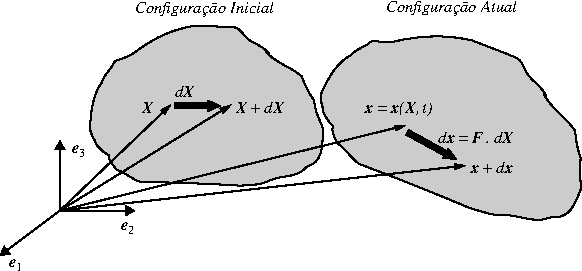
\includegraphics[scale = 1.1]{fig1-2.pdf} % Include the figure image
	\caption{Gradiente de deformação $\Fll$ e o transporte de um vetor material $d\Xl$}
	\label{fig:fig1-2.pdf} % Unique label used for referencing the figure in-text
\end{figure}

O vetor $d\xl$ pode ser obtido de $d\Xl$ pela diferenciação de (\ref{eq:Xl_e_xl}):

\begin{equation}
	\label{eq:dx_indicial}	
	d\xl = \dfrac{\partial x_i}{\partial X_j}dX_j\el_i
\end{equation}
ou, equivalentemente:
\begin{equation}
	\label{eq:dx}	
	d\xl = \Fll \cdot d\Xl
\end{equation}
onde:
\begin{equation}
	\label{eq:Fll}	
	\Fll = \nabla_X \xl ; ~~ F_{ij} = \dfrac{\partial x_i}{\partial X_j}
\end{equation}

Em (\ref{eq:Fll}) $\nabla_X$ representa o operador gradiente (nabla) relativo a configuração inicial. $\Fll$ é chamado de \textbf{gradiente de deformações}. Ele transporta qualquer vetor material $d\Xl$ em seu deformado $d\xl$. Sua inversa $\Fll^{-1}$ e sua transposta ${}^t \Fll$ são respectivamente definidos por:

\begin{equation}
	\label{eq:inversaFll_e_transpostaFll}	
	d\Xl = \Fll^{-1} \cdot d\xl; ~~ d\xl = d\Xl \cdot {}^t\Fll
\end{equation}
\footnote{N.T.: na segunda expressão de (\ref{eq:inversaFll_e_transpostaFll}) se usa a propriedade de permutação na contração simples entre um tensor de segunda ordem e de primeira ordem: $\textbf{T} \cdot \textbf{v} = \textbf{v} \cdot {}^t\textbf{T}$}e satisfazem:
\begin{equation}
	\label{eq:inversaFll_e_transpostaFll2}	
	({}^t\Fll)_{ij} = F_{ji}; ~~(\Fll^{-1})_{ij} = \dfrac{\partial X_i}{\partial x_j}
\end{equation}

\paragraph{Gradiente de deformações e deslocamento}\index{Sectioning!Paragraphs} Seja $\Xil(\Xl,t)$ o vetor deslocamento da partícula da qual a posição inicial e atual são $\Xl$ e $\xl$, respectivamente. Escrevemos:

\begin{equation}
	\label{eq:Xl+Xli}	
	\xl = \Xl + \Xil
\end{equation}

Das definições (\ref{eq:Fll}) e (\ref{eq:Xl+Xli}) o gradiente de deformação pode ser expresso como uma função do vetor deslocamentos $\Xil$ conforme \footnote{N.T.: Nessa dedução aplica-se o gradiente $\nabla_X$ em ambos os lados da equação (\ref{eq:Xl+Xli}) lembrando que o $\nabla_X \cdot \Xl = \onell$}:

\begin{equation}
	\label{eq:Fll=1+nablaXil}	
	\Fll = \onell + \nabla_X \Xil; ~~ F_{ij} = \delta_{ij}+\dfrac{\xi_i}{X_j}
\end{equation}	
onde $\delta_{ij}$ é o delta de Kronecker, que é $\delta_{ij}=1$ se $i=j$ e $\delta_{ij}=0$ se $i \neq j$.

\paragraph{Trasnporte de volume}\index{Sectioning!Paragraphs} O volume infinitesimal atual $d\Omega_t=dx_1 dx_2 dx_3$ é igual ao produto composto\footnote{N.T.: Pode-se aplicar diretamente a função determinante:
	\begin{displaymath}	
	d\Omega_t = (dx_1\el_1, dx_2\el_2, dx_3\el3) = \begin{vmatrix}
	dx_1 & 0 & 0 \\
	0	& dx_2  & 0 \\
	0	& 0 & dx_3
	\end{vmatrix} = dx_1 dx_2 dx_3	
	\end{displaymath}
}:

\begin{equation}
	\label{eq:domegat}	
	d\Omega_t = (d\xl_1, d\xl_2, d\xl_3) = d\xl_1 \cdot (d\xl_2 \times d\xl_3)
\end{equation}	
onde $d\xl_i=dx_i\el_i$ (com nenhum somatório). A lineariedade do produto composto com respeito aos vetores combinados permite nós escrevermos \footnote{N.T.: Nessa dedução deve-se usar a propriedade de quando se multiplica linhas ou colunas de um determinante por um escalar, o determinante fica multiplicado por esse escalar. Além disso, a contração $\Fll \cdot \el_i$ extrai o vetor correspondente a linha $i$ de $\Fll$.

	\begin{displaymath}	
	d\Omega_t = (dX_1 \Fll \cdot \el_1, dX_2 \Fll \cdot \el_2, dX_3 \Fll \cdot \el3) = dX_1 dX_2 dX_3(\Fll \cdot \el_1, \Fll \cdot \el_2, \Fll \cdot \el3) = dX_1 dX_2 dX_3 \det(\Fll)
\end{displaymath}

}:
\begin{equation}
	\label{eq:domegat2}	
	d\Omega_t = (\Fll \cdot d\xl_1, \Fll \cdot d\xl_2, \Fll \cdot d\xl_3) = \det (\Fll)(d\Xl_1, d\Xl_2, d\Xl_3)
\end{equation}

Como consequência qualquer volume material inicial $d\Omega_0$ se transforma no volume material $d\Omega_t$ através da relação:

\begin{equation}
	\label{eq:domegat2}	
	d\Omega_t = Jd\Omega_0
\end{equation}
onde $J=det{\Fll}$ é o Jacobiano da deformação.

\paragraph{Trasnporte de superfície}\index{Sectioning!Paragraphs} Considere uma superficie material $dA$, orientada pelo vetor unitário normal $\Nl$. Ao longo da deformação $dA$ se transforma na superfície material $da$, orientada pelo vetor normal $\nl$. Como os vetores $\Nl$ e $\nl$ não são vetores materiais, eles não sofrem deformação. Seja $\Ul$ qualquer vetor material na configuração inicial. O cilindro material de volume inicial $\Nl \cdot \Ul dA$ se transforma no cilindro material de volume $\nl \cdot \Fll \cdot \Ul da$ (ver \autoref{fig:fig1-3.pdf}). 

\begin{figure}[H] % Use [H] to suppress floating and place the figure/table exactly where it is specified in the text
	\centering % Horizontally center the figure on the page
	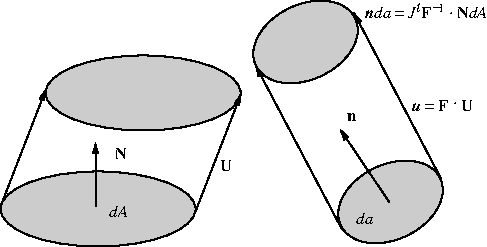
\includegraphics[scale = 1.1]{fig1-3.pdf} % Include the figure image
	\caption{Gradiente de deformação $\Fll$ e o transporte de um vetor material $d\Xl$}
	\label{fig:fig1-3.pdf} % Unique label used for referencing the figure in-text
\end{figure}


Conforme (\ref{eq:domegat2}) pode-se escrever:

\begin{equation}
	\label{eq:nFUda=JNUda}	
	\nl \cdot \Fll \cdot \Ul da = J \Nl \cdot \Ul dA
\end{equation}

Como (\ref{eq:nFUda=JNUda}) vale qualquer que seja o vetor $\Ul$, derivamos:

\begin{equation}
	\label{eq:nda=JFNdA}	
	\nl da = J {}^t\Fll \cdot \Nl dA; ~~ n_ida = J \dfrac{\partial X_j}{\partial x_i}N_jdA
\end{equation}

Seja $\vl$ qualquer vetor ligado à configuração atual e seja $\Vl$ o vetor associado ligado a configuração inicial e definido de tal forma que o fluxo de $\vl$ através de $da$ coincide com o fluxo de $\Vl$ através de $dA$. Nós escrevemos:

\begin{equation}
	\label{eq:vnda=VNdA}	
	\vl \cdot \nl da = \Vl \cdot \Nl dA;~~ v_in_ida = JV_i\dfrac{\partial X_j}{\partial x_i}N_jdA
\end{equation}

De (\ref{eq:nda=JFNdA}) e (\ref{eq:vnda=VNdA}) derivamos \footnote{N.T.: Durante essa dedução é usado a propriedade que na contração simples um tensor de primeira ordem pode ser permutado com um tensor de segunda ordem, desde que transponha o tensor de segunda ordem $\textbf{T} \cdot \textbf{v} = \textbf{v} \cdot {}^t\textbf{T}$:
	\begin{displaymath}	
	\vl \cdot \nl da = \vl \cdot J {}^t \Fll^{-1} \cdot \Nl dA = \Vl \cdot \Nl dA \iff \Vl = \vl \cdot J {}^t \Fll^{-1} \therefore  \Vl = J \Fll^{-1} \cdot \vl
	\end{displaymath}

}:

\begin{equation}
	\label{eq:V=JF-1}	
\Vl = J \Fll^{-1} \cdot \vl; ~~ V_i = J \dfrac{\partial X_i}{\partial x_j}v_j
\end{equation}

Integrando (\ref{eq:vnda=VNdA}) no volume $\Omega_0$ e $\Omega_t$ na deformação, seguida pelo uso do Teorema da Divergência e da relação (\ref{eq:domegat2}) tem-se a seguinte identidade útil \footnote{N.T.: A dedução dessa expressão:
	\begin{displaymath}	
		\vl \cdot \nl da = \Vl \cdot \Nl dA
	\end{displaymath}
	\begin{displaymath}	
	\int_{\partial \Omega_t}^{}\vl \cdot \nl da = \int_{\partial \Omega_0}^{}\Vl \cdot \Nl dA
	\end{displaymath}
	Usando o Teorema da Divergência a expressão anterior fica:
	\begin{displaymath}	
	\int_{\Omega_t}^{}\nabla_x \cdot \vl d\Omega_t = \int_{ \Omega_0}^{} \nabla_X \cdot \Vl d\Omega_0 \iff \nabla_x \cdot \vl d\Omega_t = \nabla_X \cdot \Vl d\Omega_0 \therefore J \nabla_x \cdot \vl = \nabla_X \cdot \Vl
	\end{displaymath}

}:

\begin{equation}
	\label{eq:nablaxvdOmegat=nablaXVdOmega0}	
	\nabla_x \cdot \vl d\Omega_t = \nabla_X \cdot \Vl d\Omega_0; ~~ J\dfrac{\partial v_i}{\partial x_i} = \dfrac{\partial V_i}{\partial X_i}
\end{equation}

\subsection{Porosidades Euleriana e Lagrangeana. Razão de Vazios}\index{Sectioning!Subsections}

Seja $n$ a \textbf{porosidade Euleriana}, de modo que o fluído ocupa o volume $nd\Omega_t$ na configuração atual \footnote{N.T.: A porosidade Euleriana pode ser escrita da seguinte forma:
		\begin{displaymath}
		n = \dfrac{\text{Volume poroso atual}}{\text{Volume do esqueleto atual}} = \dfrac{nd\Omega_t}{d\Omega_t} 
		\end{displaymath}}. Como o volume material do esqueleto $d\Omega_t$ muda através da deformação, a porosidade $n$ não quantifica adequadamente a mudança de volume sofrida pelo espaço poroso em relação ao volume inicial $d\Omega_0$. Ao contrário da porosidade Euleriana $n$, que se refere ao volume atual $d\Omega_t$, a mudança no espaço poroso é eventualmente melhor capturada pela \textbf{porosidade Lagrangeana} \footnote{N.T.:
	A definição da porosidade Lagrangeana leva a dedução da relação (\ref{eq:phidOmega0=ndOmegat}):
	\begin{displaymath}		
		\phi = \dfrac{\text{Volume poroso atual}}{\text{Volume do esqueleto inicial}} = \dfrac{nd\Omega_t}{d\Omega_0} \therefore \phi d\Omega_0 = n d\Omega_t \therefore \phi = n \dfrac{d\Omega_t}{d\Omega_0} \therefore \phi = Jn
	\end{displaymath}
} $\phi$, que relaciona o volume poroso atual ao volume inicial $d\Omega_0$ conforme:

\begin{equation}
	\label{eq:phidOmega0=ndOmegat}	
\phi d\Omega_0 = n d\Omega_t; ~~\phi = Jn
\end{equation}

Por sua vez, o atual grau de compacidade de um material poroso é bem capturado pela \textbf{razão de vazios} definida como a razão entre o volume poroso atual e o volume atual da matriz. Devido à sua definição, a razão de vazios $e$ é uma variável Euleriana, sem contraparte Lagrangeana, e é expresso em função de $n$ na forma \footnote{N.T.:				
	\begin{displaymath}	
		e = \dfrac{\text{Volume poroso atual}}{\text{Volume da matriz}} = \dfrac{nd\Omega_t}{d\Omega_t-nd\Omega_t} = \dfrac{n}{1-n}
	\end{displaymath}}:
\begin{equation}
	\label{eq:e}	
	e = \dfrac{n}{1-n}
\end{equation}

\subsection{Tensor de Deformações}\index{Sectioning!Subsections}

Deformação induz mudanças nos comprimentos dos vetores materiais e nos ângulos entre eles. O tensor de deformações de Green-Lagrange $\Deltall$ mede essas mudanças quantificando a variação do produto escalar entre dois vetores materiais $d\Xl$ e $d\Yl$ com relação aos mesmos deformados $d\xl$ e $d\yl$. Nós escrevemos \footnote{N.T.: 
\begin{displaymath}	
	d\xl \cdot d\yl - d\Xl \cdot d\Yl = (\Fll \cdot d\Xl) \cdot (\Fll \cdot d\Yl) -  d\Xl \cdot d\Yl
\end{displaymath}
\begin{displaymath}	
	~~~~~~~~~~~~~~~~~~~~~~~~~~~~ = (d\Xl \cdot {}^t\Fll) \cdot (\Fll \cdot d\Yl) -  d\Xl \cdot d\Yl
\end{displaymath}
\begin{displaymath}	
	~~~~~~~~~~~~~~~~~~~~~~~~~~~~ = d\Xl \cdot ({}^t\Fll \cdot \Fll \cdot d\Yl -  d\Yl)
\end{displaymath}
\begin{displaymath}	
	~~~~~~~~~~~~~~~~~~~~~~~~~~~~ = d\Xl \cdot ({}^t\Fll \cdot \Fll -  \onell) \cdot d\Yl
\end{displaymath}
\begin{displaymath}	
	~~~~~~~~~~~~~~~~~~~~~~~~~~~~ = d\Xl \cdot 2 \Deltall \cdot d\Yl
\end{displaymath}
\begin{displaymath}	
	~~~~~~~~~~~~~~~~~~~~~~~~~~~~ = 2 d\Xl \cdot \Deltall \cdot d\Yl
\end{displaymath}

O valor de 2 é um valor arbitrário.

}:
\begin{equation}
	\label{eq:dxdy}	
	d\xl = \Fll \cdot d\Xl ;  ~~ d\yl = \Fll \cdot d\Yl: ~~ d\xl \cdot d\yl - d\Xl \cdot d\Yl = 2d\Xl \cdot \Deltall \cdot d\Yl
\end{equation}

Com a ajuda de (\ref{eq:inversaFll_e_transpostaFll}) pode-se escrever como uma função do gradiente de deformações conforme \footnote{N.T.: quando se tem ${}^t\Fll \cdot \Fll = \onell$ tem-se um movimento de corpo rígido sem deformação (isometria). Pode transladar ou rotacionar, mas não se deforma. Uma rotação pura ainda adiciona a seguinte condição: $\det {\Fll}=1$. Nessa expressão pode-se ver que a deformação é o afastamento da isometria.}.

\begin{equation}
	\label{eq:Deltall}	
	\Deltall = \dfrac{1}{2}({}^t\Fll \cdot \Fll - \onell)
\end{equation}

Sendo simétrico, o tensor $\Deltall$ admite três autovalores reais $\Delta_J (J=I,II,III)$. Esses últimos são as deformações principais e estão associados com os autovetores $\el_J (J=I,II,III)$, que são as direções principais das deformações principais de modo que $\Deltall \cdot \el_J = \Delta_J \el_J$. A ortogonalidade das direções principais, escrita $\el_I \cdot \el_J = 0$, é preservada na deformação. De fato:

\begin{equation}
	\label{eq:eIFFeJ}	
	(\el_I \cdot {}^t \Fll) \cdot (\Fll \cdot \el_J) = 2\el_I \cdot \Deltall \cdot \el_J = 2 \Delta_{I~\text{ou}~J} \el_I \cdot \el_J = 0
\end{equation}

O gradiente $\Rll$ da rotação que rigidamente transporta o conjunto de direções principais ortogonais $\el_J$ para sua direção final é uma isometria de modo que o tensor de deformações é nulo, resultando em ${}^t\Rll = \Rll^{-1}$. Portanto, o gradiente $\Fll$ de qualquer transformação pode ser decomposto como:

\begin{equation}
	\label{eq:F=DR}	
	\Fll = \Dll \cdot \Rll
\end{equation}

que é a rotação $\Rll$ seguida pela deformação atual $\Dll$, esta última envolvendo nenhuma rotação e correspondendo à dilatação das direções principais de deformação. Equivalentemente, o gradiente $\Fll$ pode se decompor como a atual deformação $\Dll'$ correspondente à dilatação, seguido por uma rotação $\Rll'$ relativo aos autovetores. Assim, o tensor de deformações $\Deltall$ leva em conta inteiramente a deformação atual, uma vez que \footnote{
N.T.: Nessa dedução é utilizado as seguintes propriedades dos tensores de segunda ordem na contração simples: $(\Tll \cdot \Tll') = ({}^t\Tll' \cdot \Tll)$ e ${}^t(\Tll \cdot \Tll') =({}^t\Tll' \cdot {}^t\Tll)$. Além disso, devido a ortogonalidade da matriz de rotação tem-se $\Rll \cdot {}^t\Rll = {}^t\Rll \cdot {}^t\Rll = \onell$ de modo que:
\begin{displaymath}	
	\Deltall = \dfrac{1}{2}({}^t\Fll \cdot \Fll - \onell)
\end{displaymath}
\begin{displaymath}	
	~~~~ = \dfrac{1}{2}({}^t\Rll \cdot {}^t\Dll \cdot \Dll \cdot \Rll - \onell)
\end{displaymath}
\begin{displaymath}	
	~~~~ = \dfrac{1}{2}(\Dll \cdot \Rll^t \cdot {}^t\Rll \cdot \Dll - \onell)
\end{displaymath}
\begin{displaymath}	
	~~~~ = \dfrac{1}{2}(\Dll \cdot \onell \cdot \Dll - \onell)
\end{displaymath}
\begin{displaymath}	
	~~~~ = \dfrac{1}{2}(\Dll^2- \onell)
\end{displaymath}

}:

\begin{equation}
	\label{eq:Deltall = 1/2(D^2-1)}	
	\Deltall = \dfrac{1}{2}(\Dll^2 - \onell)
\end{equation}

Por meio de (\ref{eq:Fll=1+nablaXil}) $\Deltall$ pode finalmente ser expresso como uma função do vetor de deslocamentos $\Xil$, conforme \footnote{N.T.: Nessa dedução utiliza-se a propriedade distributiva da contração simples.

\begin{displaymath}	
	\Deltall = \dfrac{1}{2}({}^t\Fll \cdot \Fll - \onell)
\end{displaymath}
\begin{displaymath}	
	\Deltall = \dfrac{1}{2}[(\onell+{}^t\nabla_X\Xil) \cdot (\onell+\nabla_X\Xil) - \onell]
\end{displaymath}
\begin{displaymath}	
	\Deltall = \dfrac{1}{2}[\onell+\nabla_X\Xil+{}^t\nabla_X\Xil+ {}^t\nabla_X\Xil \cdot \nabla_X\Xil - \onell] = \dfrac{1}{2}(\nabla_X \Xil + {}^t\nabla_X \Xil+{}^t\nabla_X \Xil \cdot \nabla_X \Xil)
\end{displaymath}

}:

\begin{equation}
	\label{eq:Deltall2}	
	\Deltall = \dfrac{1}{2}(\nabla_X \Xil + {}^t\nabla_X \Xil+{}^t\nabla_X \Xil \cdot \nabla_X \Xil) ;~~ \Delta_{ij}=~\dfrac{1}{2}\left( \dfrac{\partial \xi_i}{\partial X_j} + \dfrac{\partial \xi_j}{\partial X_i} + \dfrac{\partial \xi_k}{\partial X_i} \dfrac{\partial \xi_k}{\partial X_j} \right)
\end{equation}


\subsection{Transformações infinitesimais e linearização do tensor de deformações}\index{Sectioning!Subsections}

Em muitos problemas uma aproximação de primeira ordem da teoria finita pode ser feita sobre condições de transformações infinitesimais, ou seja:

\begin{equation}
	\label{eq:HTI}	
	\| \nabla \Xil \| \ll 1
\end{equation}

onde a norma $\|(\cdot)\|$ de $(\cdot)$ não foi especificada devido à equivalência de todas as normas no espaço vetorial de três dimensões finitas. Além disso, no que diz respeito apenas às derivações espaciais, no limite da transformação infinitesimal as configurações atual e inicial se fundem e o operador nabla $\nabla$ pode ser usado sem a necessidade de um subscrito referindo-se a uma configuração particular, ou seja $\nabla = \nabla_X \equiv \nabla_x$.

Sobre a condição de (\ref{eq:HTI}) o tensor de deformações de Green-Lagrange $\Deltall$ se reduz ao tensor de deformações linearizado $\strainll$: 

\begin{equation}
	\label{eq:strainll}
\Deltall \simeq \strainll = \dfrac{1}{2}(\nabla \Xil + {}^t\nabla \Xil); ~~ \varepsilon_{ij} =  \dfrac{\partial \xi_i}{\partial x_j} + \dfrac{\partial \xi_j}{\partial x_i}
\end{equation}

Uma vez que $\Deltall$ tem a mesma ordem de magnitude que $\nabla_X\Xil$, a transformação infinitesimal implica deformação infinitesimal, ou seja $\|\Deltall\| \ll 1$. Porém, a deformação pode ser infinitesimal enquanto que a transformação não é. Por exemplo, no movimento de corpo rígido $\Deltall$ é nulo enquanto que $\nabla_X \Xil$ pode ter qualquer odem de magnitude.

Com a aproximação das transformações infinitesimais, (\ref{eq:Fll=1+nablaXil}) fornece \footnote{N.T.: Na hipótese das transformações infinitesimais, ao fazer o determinante os termos multiplicativos de mais alta ordem tendem a zero:
\begin{displaymath}		
\det(\Fll) = \det (\onell + \nabla \Xil) = \begin{vmatrix}
	1+\dfrac{\partial \xi_1}{\partial x_1} & \dfrac{\partial \xi_1}{\partial x_2} & \dfrac{\partial \xi_1}{\partial x_3} \\
	\dfrac{\partial \xi_2}{\partial x_1} & 1 + \dfrac{\partial \xi_2}{\partial x_2} & \dfrac{\partial \xi_2}{\partial x_3} \\
	\dfrac{\partial \xi_3}{\partial x_3} & \dfrac{\partial \xi_2}{\partial x_3} & 1+ \dfrac{\partial \xi_3}{\partial x_3}
\end{vmatrix} = 1 + \dfrac{\partial \xi_1}{\partial x_1} + \dfrac{\partial \xi_2}{\partial x_2} + \dfrac{\partial \xi_3}{\partial x_3} = 1 + \text{tr}(\strainll) = 1 + \nabla \cdot \Xil
\end{displaymath}	}:

\begin{equation}
	\label{eq:J}	
	\left(J = \det \Fll\right) \simeq \left(1+\nabla \cdot \Xil = 1 + \dfrac{\partial \xi_i}{\partial x_i} = 1 + \varepsilon_{ii}\right)
\end{equation}

De agora em diante, seja $\epsilon$ a dilatação volumétrica linearizada do esqueleto, ou seja:

\begin{equation}
	\label{eq:epsilon}	
	\epsilon = \varepsilon_{ii} = \nabla \cdot \Xil
\end{equation}
de modo que (\ref{eq:domegat2}) toma a forma de:
\begin{equation}
	\label{eq:domegatlinearizado}	
	d\Omega_t \simeq (1+\epsilon)d\Omega_0
\end{equation}

A dilatação volumétrica macroscópica observavel sofrida pelo esqueleto se deve tanto à mudança de porosidade e a dilatação $\epsilon_s$ sofrida pela matriz sólida, embora esta última não seja acessível a partir de experimentos puramente macroscópicos. Analogamente a (\ref{eq:domegatlinearizado}) a definição de $\epsilon_s$ nos permite escrever:

\begin{equation}
	\label{eq:domegats}	
	d\Omega_t^s = (1+\epsilon_s)d\Omega_0^s
\end{equation}

Devido a respectiva definição da porosidade Euleriana e Lagrangiana, $n$ e $\phi$, o volume ocupado pela matriz é vinculado ao volume total através da relação:

\begin{equation}
	\label{eq:domegats2}	
	d\Omega_t^s = (1-n)d\Omega_t = d\Omega_t - \phi d\Omega_0; ~~~ d\Omega_0^s = (1-\phi_0)d\Omega_0
\end{equation}

Combinando as equações acima, nós finalmente derivamos o balanço de volume \footnote{N.T.: dedução: \\ Igualando (\ref{eq:domegats}) e (\ref{eq:domegats2}): $(1+\epsilon_s)d\Omega_0^s = d\Omega_t - \phi d\Omega_0$. \\ Colocando $d\Omega_0^s$ de (\ref{eq:domegats2}): $(1+\epsilon_s)(1-\phi_0)d\Omega_0 = d\Omega_t - \phi d\Omega_0$.\\ Dividindo ambos lados da igualdade por $d\Omega_0$: $(1+\epsilon_s)(1-\phi_0) = \frac{d\Omega_t}{d\Omega_0} - \phi$
. \\ Colocando $\frac{d\Omega_t}{d\Omega_0}$ de (\ref{eq:domegatlinearizado}) tem-se: $(1+\epsilon_s)(1-\phi_0) = 1+\epsilon - \phi$ que rearranjando leva a: $\epsilon = (1-\phi_0)\epsilon_s + \phi - \phi_0$
}:

\begin{equation}
	\label{eq:epsilongraocompressivel}	
	\epsilon = (1-\phi_0)\epsilon_s + \phi - \phi_0
\end{equation}

Na ausência de porosidade oclusa, os grãos do sólido que formam a matriz sofrem mudanças de volumes desprezíveis de modo que a matriz pode ser considerada incompressível. Assim fazemos $\epsilon_s = 0$ em (\ref{eq:epsilongraocompressivel}), obtendo:

\begin{equation}
	\label{eq:epsilon}	
	\epsilon = \phi - \phi_0
\end{equation}

Como geralmente é feito na mecânica dos solos, pode ser mais conveniente usar a razão de vazios em vez da dilatação volumétrica. Combinando (\ref{eq:phidOmega0=ndOmegat}), (\ref{eq:e}) e (\ref{eq:epsilon}) obtemos \footnote{N.T.: tem-se que:
	\begin{displaymath}	
		\phi = \dfrac{e}{1+e_0} ~~~ \text{e} ~~~ \phi_0 = \dfrac{e_0}{1+e_0} ~~~ \text{e portanto}  ~~~ \epsilon = \phi - \phi_0 = \dfrac{e-e_0}{1+e_0}
	\end{displaymath}
}:

\begin{equation}
	\label{eq:epsilon}	
	\epsilon = \dfrac{e-e_0}{1+e_0}
\end{equation}

Sobre a aproximação das transformações infinitesimais, o termo da diagonal $\varepsilon_{ii}$ (sem somatório) é igual a dilatação linear na direção $\el_i$, enquanto que o termo duplo fora da diagonal, $\gamma_{ij}=2\varepsilon_{ij}~(i\neq j)$, é igual a distorção relacionada com as direções $\el_i$ e $\el_j$ que estavam normais antes da deformação.


\section{Cinemática}\index{Sectioning!Sections}

A descrição da deformação do esqueleto por meio do gradiente de deformação $\Fll$ é por natureza uma descrição Lagrangiana. Os campos são funções do tempo $t$ e do vetor posição $\Xl$ localizando a partícula do esqueleto na configuração inicial. A posição $\Xl$ não varia com o tempo e a cinemática do esqueleto resulta de uma simples derivação.

Em contraste a abordagem Lagrangeana, a abordagem Euleriana envolve apenas a configuração atual, sem referência a qualquer configuração inicial. A abordagem é feita usando o campo de velocidades $\Vl^\pi(\xl,t)$ da particula coincidindo no tempo $t$ com a geometria do ponto localizado em $\xl$. A partícula pode ser uma partícula de esqueleto, $\pi = s$, ou uma partícula de fluído, $\pi = f$\footnote{Teria sido mais rigoroso fazer uma distinção entre o índice referente ao assunto na escala macroscópica (por exemplo, $sk$ para a partícula do esqueleto e $fl$ para a partícula de fluído) e o índice referindo a matéria na mesoescala (por exemplo, $s$ para a matriz sólida, como em (\ref{eq:epsilongraocompressivel}), e $f$ para o fluído). Contudo, por uma questão de simplicidade da notação, optamos por não fazer essa distinção}. No tempo $t$, a mesma abordagem Euleriana se aplica a ambas as partículas, pois o esqueleto contínuo e o fluído contínuo se fundem na mesma configuração atual.

\subsection{Derivada Material}\index{Sectioning!Subsections}
\textbf{Definição}
A derivada material $d^\pi \mathcal{G}/dt$ com relação a partícula $\pi$ ($=s$ ou $f$) de algum campo $\mathcal{G}$ é a derivada temporal de $G$ que um observador ligado a partícula derivaria. Este observador registra a variação $d^\pi\mathcal{G}$ da quantidade $\mathcal{G}$ entre os tempos $t$ e $t+dt$. Por exemplo, sendo a origem de coordenadas fixa, o campo de velocidades $\Vl^\pi(\xl,t)$ da partícula $\pi$ localizada a $\xl$ se lê:

\begin{equation}
	\label{eq:dpix1}	
	\dfrac{d^\pi\xl}{dt} = \Vl^\pi(\xl,t); ~~~ \pi = s ~~\text{ou} ~~~f
\end{equation}
\textbf{Derivada material de um vetor material}

A definição (\ref{eq:dpix1}) nos permite escrever a derivada material de um vetor material $d\xl$ na forma:

\begin{equation}
	\label{eq:dpix2}	
	\dfrac{d^\pi}{dt}(d\xl) = \dfrac{d^\pi}{dt}[(\xl+d\xl)-\xl]=\Vl^\pi(\xl+d\xl,t)- \Vl^\pi(\xl,t) 
\end{equation}

de modo que:

\begin{equation}
	\label{eq:dpix3}	
	\dfrac{d^\pi}{dt}(d\xl) = \nabla_x\Vl^\pi \cdot d\xl; ~~ (\nabla_x \Vl^\pi)_{ij} = \dfrac{\partial V_i^\pi}{\partial x_j}; ~~ \pi = s ~~ \text{ou} ~~ f
\end{equation}

\textbf{Derivada material de um volume material}

Iniciando de (\ref{eq:domegat}) nós podemos expressar a derivada material de um volume material $d\Omega_t$ na forma:

\begin{equation}
	\label{eq:derivadavolumematerial}	
	\dfrac{d^\pi}{dt}(d\Omega_t) = \dfrac{d^\pi}{dt}(d\xl_1,d\xl_2,d\xl_3) = \dfrac{d^\pi}{dt}(d\xl_1\cdot (d\xl_2 \times d\xl_3))
\end{equation}

A linearidade do produto composto $(\vl_1, \vl_2, \vl_3)$ com respeito aos vetores $\vl_{i=1,2,3}$ nos permite escrever: 

\begin{equation}
	\label{eq:derivadavolumematerial1}	
	\dfrac{d^\pi}{dt}(d\Omega_t) = \left(\dfrac{d^\pi}{dt}(d\xl_1),d\xl_2,d\xl_3\right) + \left(d\xl_1,\dfrac{d^\pi}{dt}(d\xl_2),d\xl_3\right)+\left(d\xl_1,d\xl_2,\dfrac{d^\pi}{dt}(d\xl_3)\right)
\end{equation}

Usando (\ref{eq:dpix3}) obtém-se:

\begin{equation}
	\label{eq:derivadavolumematerial2}	
	\dfrac{d^\pi}{dt}(d\Omega_t) = \left(\dfrac{\partial V_i^\pi}{\partial x_1}\el_idx_1,d\xl_2,d\xl_3\right) + \left(d\xl_1,\dfrac{\partial V_i^\pi}{\partial x_2}\el_idx_2,d\xl_3\right)+\left(d\xl_1,d\xl_2,\dfrac{\partial V_i^\pi}{\partial x_3}\el_idx_3\right)
\end{equation}

O produto $(\vl_1,\vl_2,\vl_3)$ é zero assim que dois vetores entre os vetores $\vl_{i=1,2,3}$ são colineares. Portanto:

\begin{equation}
	\label{eq:derivadavolumematerial3}	
	\dfrac{d^\pi}{dt}(d\Omega_t) = \left(\dfrac{\partial V_1^\pi}{\partial x_1},\dfrac{\partial V_2^\pi}{\partial x_2},\dfrac{\partial V_3^\pi}{\partial x_3}\right)(d\xl_1,d\xl_2,d\xl_3)
\end{equation}
ou equivalentemente:
\begin{equation}
	\label{eq:derivadavolumematerial3}	
	\dfrac{d^\pi}{dt}(d\Omega_t) = (\nabla_x \cdot \Vl^\pi)d\Omega_t; ~~~ \pi = s ~~\text{ou} ~~ f
\end{equation}

\textbf{Derivada material de um campo}

A derivada material $d^\pi \mathcal{G}/dt$ com respeito a partícula $\pi (=s~~\text{ou}~~f)$ do campo $\mathcal{G}(\xl, t)$ vem a ser a derivada de tempo de $\mathcal{G}$ ao deixar $\xl$ coincidir com as sucessivas posições $\xl^{\pi}(t)$ ocupadas pela partícula. Nós escrevemos:

\begin{equation}
	\label{eq:derivadavolumematerial4}	
	\frac{d^\pi \mathcal{G}}{dt} = \dfrac{\partial \mathcal{G}}{\partial t} + (\nabla_x \mathcal{G} \cdot \Vl^{\pi})
\end{equation}

Por exemplo, a aceleração $\gammal^{\pi}$ da partícula $\pi$ é a derivada material da velocidade $\Vl^{\pi}(\xl,t)$:

\begin{equation}
	\label{eq:derivadavolumematerial5}	
	\gammal^{\pi} = \dfrac{d^\pi \Vl^{\pi}}{dt} = \dfrac{\partial \Vl^{\pi}}{\partial t}+(\nabla_x \Vl^{\pi})\cdot \Vl^\pi
\end{equation}

\textbf{Derivada material de um volume integral}

A derivada material se aplica à integral de volume de qualquer quantidade $\mathcal{G}$ confome:

\begin{equation}
	\label{eq:derivadavolumematerial6}	
	\dfrac{d^\pi}{dt}\int_{\Omega_t}\mathcal{G}d\Omega_t = \int_{\Omega_t}\dfrac{d^\pi}{dt}(\mathcal{G}d\Omega_t)
\end{equation}

Com o uso de (\ref{eq:derivadavolumematerial3}) e (\ref{eq:derivadavolumematerial4}) nos permite reescrever (\ref{eq:derivadavolumematerial6}) na forma:

\begin{equation}
	\label{eq:derivadavolumematerial7}	
	\dfrac{d^\pi}{dt}\int_{\Omega_t}\mathcal{G}d\Omega_t = \int_{\Omega_t}\left(\dfrac{\partial^\pi \mathcal{G}}{\partial t}+\mathcal{G}\nabla_x \cdot \Vl^{\pi}\right)d\Omega_t
\end{equation}

ou, equivalentemente:

\begin{equation}
	\label{eq:derivadavolumematerial8}	
	\dfrac{d^\pi}{dt}\int_{\Omega_t}\mathcal{G}d\Omega_t = \int_{\Omega_t}\left(\dfrac{\partial^\pi \mathcal{G}}{\partial t}+\nabla_x \cdot (\mathcal{G}\Vl^{\pi})\right)d\Omega_t
\end{equation}

Usando o teorema da divergência finalmente tem-se a expressão alternativa:

\begin{equation}
	\label{eq:derivadavolumematerial9}	
	\dfrac{d^\pi}{dt}\int_{\Omega_t}\mathcal{G}d\Omega_t = \int_{\Omega_t}\dfrac{\partial^\pi \mathcal{G}}{\partial t}d\Omega_t+\int_{\partial \Omega_t} \mathcal{G}\Vl^{\pi} \cdot \nl da
\end{equation}
em que $\partial \Omega t$ é a borda do volume $\Omega_t$ enquanto que $\nl$ é o vetor normal que aponta para fora da superfície $da$.

\subsection{Taxa de deformação}\index{Sectioning!Subsections}

A derivada material permite a descrição Euleriana da cinemática da deformação que se refere apenas a configuração atual. A taxa Euleriana do tensor de deformações é definida pela relação:

\begin{equation}
	\label{eq:taxadedeformacaoeuleriana1}	
	\dfrac{d^\pi}{dt}(d\xl \cdot d\yl) = 2d\xl \cdot \dl^{\pi} \cdot d\yl
\end{equation}
em que $d\xl$ e $d\yl$ são quaisquer vetores materiais do esqueleto ($\pi = s$) ou do fluído ($\pi = f$). Usando de (\ref{eq:dpix3}) em (\ref{eq:taxadedeformacaoeuleriana1}) tem-se: 

\begin{equation}
	\label{eq:taxadedeformacaoeuleriana2}	
\dl^{\pi} = \dfrac{1}{2}(\nabla_x \Vl^{\pi} + ^{t}\nabla_x \Vl^{\pi}); ~~ d^\pi_{ij} =  \dfrac{1}{2} \left(\dfrac{\partial V_i^\pi}{\partial x_j} + \dfrac{\partial V_j^\pi}{\partial x_i}\right)
\end{equation}

A definição (\ref{eq:taxadedeformacaoeuleriana2}) de $\dl^{\pi}$ nos permite decompor a deformação cinemática do vator material $d\xl$ na forma:

\begin{equation}
	\label{eq:taxadedeformacaoeuleriana3}	
	\dfrac{d^\pi}{dt}(d\xl) = \Omegall^\pi \cdot d\xl + \dl^\pi \cdot d\xl
\end{equation}
onde o $\Omegall^\pi$ é o tensor da taxa de rotação ligada a parte antissimétrica de $\nabla_x \Vl^\pi$:

\begin{equation}
	\label{eq:taxadedeformacaoeuleriana4}	
\Omegall^\pi = \dfrac{1}{2}(\nabla_x \Vl^{\pi} - ^{t}\nabla_x \Vl^{\pi}); ~~~ \Omega^\pi_{ij} = \dfrac{1}{2}\left(\dfrac{\partial V_i^\pi}{\partial x_j}-\dfrac{\partial V_j^\pi}{\partial x_i} \right)
\end{equation}

O termo $\Omegall^\pi \cdot d\xl$ em (\ref{eq:taxadedeformacaoeuleriana3}) não gera taxa de deformação uma vez que leva em conta a rotação infinitesimal do vetor material $d\xl$ conforme:

\begin{equation}
	\label{eq:taxadedeformacaoeuleriana5}	
	\Omegall^\pi \cdot d\xl = 2 \omegal^\pi \times d\xl
\end{equation}
onde $\omegal^\pi$ é o vetor vorticidade:
\begin{equation}
	\label{eq:vetorvorticidade}	
	\omegal^\pi = \nabla_x \times \Vl^\pi
\end{equation}

A decomposição Euleriana (\ref{eq:taxadedeformacaoeuleriana3}) da cinemática da deformação deve ser comparada com a decomposição Lagrangeana (\ref{eq:F=DR}) da deformação.

Em contraste com a abordagem Euleriana para a cinemática da deformação do esqueleto, a abordagem Lagrangeana consiste em derivar (\ref{eq:dxdy}) em relação ao tempo \footnote{Ao tomar a derivada material do esqueleto das quantidades Lagrangeanas, como por exemplo, $d\Deltall/dt$, vamos adotar uma notação padrão de derivada no tempo, como por exemplo, $d\Deltall/dt$ em (\ref{eq:derivadalagrangeanadeltall}). De fato, não há ambiguidade uma vez que $\Deltall = \Deltall(\Xl,t)$. Além disso, a derivada material com respeito ao fluído de uma quantidade Lagrangeana geralmente não apresenta qualquer interesse físico}:

\begin{equation}
	\label{eq:derivadalagrangeanadeltall}	
	\dfrac{d^s}{dt}(d\xl \cdot d\yl) = 2d\Xl \cdot \dfrac{d\Deltall}{dt} \cdot d\Yl
\end{equation}

Usando a formula de transporte $d\xl = \Fll \cdot d\Xl$ e $d\yl = \Fll \cdot d\Yl$, a comparação entre (\ref{eq:taxadedeformacaoeuleriana1}) para $\pi = s$ e (\ref{eq:derivadalagrangeanadeltall}) leva a seguinte fórmula de transporte:

\begin{equation}
	\label{eq:derivadalagrangeanadeltall2}	
	\dl^s = ^{t}\Fll^{-1} \cdot \dfrac{d\Deltall}{dt} \cdot \Fll^{-1}; ~~~ d_{ij}^s = \dfrac{\partial X_k}{\partial x_i}\dfrac{d\Delta_{kl}}{dt}\dfrac{\partial X_l}{\partial x_j}
\end{equation}

De acordo com (\ref{eq:strainll}) e (\ref{eq:derivadalagrangeanadeltall2}), a aproximação da transformação infinitesimal leva a considerar $d^s \simeq d\strainll/dt$

\section{Balanço de Massa}\index{Sectioning!Sections}

\subsection{Equação da Continuidade}\index{Sectioning!Subsections}

Sejam $\rho_s$ e $\rho_f$ a densidade mesoscópica ou intrínseca da matriz e do fluído de modo que $\rho_s(1-n)d\Omega_t$ e $\rho_f n d\Omega_t$ são as respectivas massas do esqueleto e do fluído atuais contidas no volume material $d\Omega_t$. Assim a densidade macroscópica ou aparente do esqueleto e do fluído são respectivamente $\rho_s(1-n)$ e $\rho_f n$. Quando não ocorre mudança de massa, nem para o esqueleto e nem para o fluído contido no volume $\Omega_t$, o balanço de massa pode ser escrito na forma:

\begin{equation}
	\label{eq:balanco_de_massa1}	
	\dfrac{d^s}{dt}\int_{\Omega_t}\rho_s(1-n)d\Omega_t = 0~~~ \text{and}~~~\dfrac{d^f}{dt}\int_{\Omega_t}\rho_fnd\Omega_t = 0 
\end{equation}

Aplicando (\ref{eq:derivadavolumematerial6}) e (\ref{eq:derivadavolumematerial8}) em (\ref{eq:balanco_de_massa1}) obtemos:

\begin{equation}
	\label{eq:balanco_de_massa2}	
	\dfrac{d^s}{dt}(\rho_s(1-n)d\Omega_t) = 0~~~ \text{e}~~~\dfrac{d^f}{dt}(\rho_fnd\Omega_t) = 0 
\end{equation}
e as equações de continuidade Euleriana:
\begin{equation}
	\label{eq:balanco_de_massa3}	
	\dfrac{\partial(\rho_s(1-n))}{\partial t} + \nabla_x \cdot (\rho_s(1-n)\Vl^s)=0 ~~~~ \text{e} ~~~~ \dfrac{\partial(\rho_fn)}{\partial t} + \nabla_x \cdot (\rho_fn\Vl^f)=0
\end{equation}

\subsection{Vetor de fluxo relativo de uma massa fluída. Vetor de Infiltração. Conteúdo de massa fluída}\index{Sectioning!Subsections}

A formulação apropriada das equações constitutivas para o esqueleto que representa os acoplamentos esqueleto-fluído exigirão a referência do movimento do fluído à configuração inicial do esqueleto. Com esse propósito em mente, seja $J_fda$ a massa do fluído entre o tempo $t$ e $t+dt$ através da superfície material do esqueleto infinitesimal $da$ orientada por um vetor normal $n$. Escrevemos: 

\begin{equation}
	\label{eq:fluxo relativo1}	J_fda = \wl \cdot \nl da
\end{equation}
em que $\wl(\xl,t)$ é o vetor Euleriano de fluxo relativo de massa fluída. Uma vez que a quantidade $n(\Vl^f-\Vl^s)\cdot \nl dadt$ é o volume infinitesimal de fluído fluindo através da superfície de esqueleto $da$ durante um tempo infinitesimal $dt$ (ver \autoref{fig:fig1-4.pdf}), o vetor relativo de massa fluída $\wl$ é consistentemente definido por:

\begin{equation}
	\label{eq:fluxo relativo1}	
	\wl = \rho_f V; ~~~~ V = n(\Vl^f-\Vl^s)
\end{equation}
onde $V$ é o vetor de infiltração. 

\begin{figure}[H] % Use [H] to suppress floating and place the figure/table exactly where it is specified in the text
	\centering % Horizontally center the figure on the page
	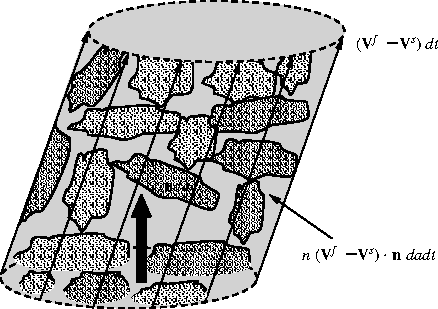
\includegraphics[scale = 1.1]{fig1-4.pdf} % Include the figure image
	\caption{Gradiente de deformação $\Fll$ e o transporte de um vetor material $d\Xl$}
	\label{fig:fig1-4.pdf} % Unique label used for referencing the figure in-text
\end{figure}

Uso da definição (\ref{eq:fluxo relativo1}) nos permite referir ao movimento do balanço de massa do fluído e do esqueleto rearranjando a equação da continuidade (\ref{eq:balanco_de_massa3})$_b$ na forma:
\begin{equation}
	\label{eq:fluxo relativo1}	
	\dfrac{d^s(\rho_fn)}{dt}+\rho_fn\nabla_x \cdot \Vl^s + \nabla_x \cdot \wl = 0 
\end{equation}

A abordagem Lagrangeana para o balanço de massa fluída pode ser realizada introduzindo o conteúdo de massa fluída Lagrangeana atual $m_f$ por unidade de volume inicial $d\Omega_0$. Esse último refere-se ao conteúdo de massa fluída Euleriana atual $\rho_fn$ por unidade de volume atual $d\Omega_t$ de acordo com:

\begin{equation}
	\label{eq:fluxo relativo2}	
	\rho_f n d\Omega_t = m_f d\Omega_0
\end{equation}

O uso de (\ref{eq:phidOmega0=ndOmegat}) e (\ref{eq:fluxo relativo2}) nos da uma relação útil:
\begin{equation}
	\label{eq:fluxo relativo3}	
	m_f = \rho_f \phi
\end{equation}
em que $\phi$ é a porosidade Lagrangeana. Além disso, seja $\Ml(\Xl,t)$ o vetor Lagrangiano anexado a configuração inicial e ligado ao vetor $\wl$ através da relação:

\begin{equation}
	\label{eq:fluxo relativo3}	
	\wl \cdot \nl da = \Ml \cdot \Nl dA
\end{equation}
onde as superfícies $da$ e $dA$ correspondem na deformação do esqueleto. Assim, fazendo com que $\wl=\vl$ e $\Ml = \Vl$ em (\ref{eq:vnda=VNdA}), Eqs. (\ref{eq:V=JF-1}) e (\ref{eq:nablaxvdOmegat=nablaXVdOmega0}) provem a seguinte fórmula de transporte:

\begin{equation}
	\label{eq:fluxo relativo4}	
	\Ml = J\Fll^{-1} \cdot \wl;~~~~ \nabla_x \cdot \wl d\Omega_t = \nabla_X \cdot \Ml d\Omega_0
\end{equation}

Substituindo (\ref{eq:fluxo relativo2}) e (\ref{eq:fluxo relativo4}) em (\ref{eq:fluxo relativo1}) pré-multiplicando por $d\Omega_t$ e usando de (\ref{eq:derivadavolumematerial3}) com $\pi = s$, obtem-se a equação Lagrangiana da continuidade na forma:

\begin{equation}
	\label{eq:fluxo relativo5}	
	\dfrac{dm_f}{dt} + \nabla_X \cdot \Ml = 0; ~~~~ \dfrac{\partial m_f(\Xl,t)}{\partial t} + \dfrac{\partial M_i}{\partial X_i} = 0
\end{equation}

Analogamente, a abordagem Lagrangiana do balanço de massa do esqueleto vem pela integração de (\ref{eq:balanco_de_massa2})$_a$ na forma:

\begin{equation}
	\label{eq:fluxo relativo6}	
	\rho_s(1-n)d\Omega_t = \rho_s^0(1-n_0)d\Omega_0
\end{equation}
em que $\rho_s^0 e n_0 = \phi_0$ representam, respectivamente, a denisidade da matriz inicial e a porosidade incial. O uso de (\ref{eq:domegat2}) nos permite escrever:
\begin{equation}
	\label{eq:fluxo relativo7}	
	m_s = m_s^0 = \rho_s^0(1-\phi_0)
\end{equation}
onde $m_s = J\rho_s(1-n)$ é o conteúdo de massa por unidade de volume inicial $d\Omega_0$ e permanece constante igual ao seu valor inicial $m_s^0$ representando a densidade do esqueleto $(\rho_s^0(1-\phi_0)$. As equações (\ref{eq:fluxo relativo5}) e (\ref{eq:fluxo relativo7}) constituem as equações Lagrangianas alternativas à  equação da continuidade Euleriana (\ref{eq:balanco_de_massa3}).

\section{Análise Avançada}\index{Sectioning!Sections}

\subsection{Derivada material com uma superfície de descontinuidade}\index{Sectioning!Subsections}
\subsection{Balanço de massa com uma superfície de descontinuidade. A condição de pulo de Rankine-Hugoniot}\index{Sectioning!Subsections}
\subsection{Balanço de massa e a rede de dupla porosidade}\index{Sectioning!Subsections}


\chapter{Capítulo 2 - Balanço de Momento. Tensor de tensões}\index{Sectioning}

Esse capítulo é dedicado a formulação do balanço de momento para um contínuo poroso visto como uma superposição de dois contínuos em interação mecânica. Tal como na Mecânica do Contínuo padrão, a existência de um tensor de tensão total simétrico e a equação do balanço de momento local em relação ao contínuo poroso visto como um todo podem ser derivados do saldo global do balanço de momento. No entanto, a derivação de equações de balanço de momento separada para o esqueleto e para o fluído não podem ser realizadas a partir de uma abordagem estritamente macroscópica. Um primeiro passo para a equação de momento em falta e um entendimento do balanço de energia mecânica envolvida no teorema da energia cinética consiste em envolver a escala mesoscópica através da introdução de tensões parciais relacionadas com cada contínuo.

\section{Balanço de Momento}\index{Sectioning!Sections}

\newcommand{\fl}{\textbf{f}}

\subsection{A hipótese de forças locais}\index{Sectioning!Subsections}

Na mecânica do contínuo qualquer domínio material $\Omega_t$ está sujeito a dois tipos de forças externas, a força externa de corpo e forças externas de superfície, como desenhado na FIGURA 2.1. Na maioria das aplicações, a força externa de corpo, tal como aquelas devido a gravidade, são as mesmas para o esqueleto e para o fluído. A força de corpo infinitesimal $\delta \fl$



\newpage

%------------------------------------------------

\section*{Unnumbered Section}

\subsection*{Unnumbered Subsection}

\subsubsection*{Unnumbered Subsubsection}

%----------------------------------------------------------------------------------------
%	IN-TEXT ELEMENT EXAMPLES CHAPTER
%----------------------------------------------------------------------------------------

\chapter{In-text Element Examples}

\section{Referencing Publications}\index{Citation}

This statement requires citation \cite{Smith:2022jd}; this one is more specific \cite[162]{Smith:2021qr}.

%------------------------------------------------

\section{Link Examples}\index{Links}

This is a URL link: \href{https://www.latextemplates.com}{LaTeX Templates}. This is an email link: \href{mailto:example@example.com}{example@example.com}. This is a monospaced URL link: \url{https://www.LaTeXTemplates.com}.

%------------------------------------------------

\section{Lists}\index{Lists}

Lists are useful to present information in a concise and/or ordered way.

\subsection{Numbered List}\index{Lists!Numbered List}

\begin{enumerate}
	\item First numbered item
	\begin{enumerate}
		\item First indented numbered item
		\item Second indented numbered item
		\begin{enumerate}
			\item First second-level indented numbered item
		\end{enumerate}
	\end{enumerate}
	\item Second numbered item
	\item Third numbered item
\end{enumerate}

\subsection{Bullet Point List}\index{Lists!Bullet Points}

\begin{itemize}
	\item First bullet point item
	\begin{itemize}
		\item First indented bullet point item
		\item Second indented bullet point item
		\begin{itemize}
			\item First second-level indented bullet point item
		\end{itemize}
	\end{itemize}
	\item Second bullet point item
	\item Third bullet point item
\end{itemize}

\subsection{Descriptions and Definitions}\index{Lists!Descriptions and Definitions}

\begin{description}
	\item[Name] Description
	\item[Word] Definition
	\item[Comment] Elaboration
\end{description}

%------------------------------------------------

\section{International Support}

àáâäãåèéêëìíîïòóôöõøùúûüÿýñçčšž

\noindent ÀÁÂÄÃÅÈÉÊËÌÍÎÏÒÓÔÖÕØÙÚÛÜŸÝÑ

\noindent ßÇŒÆČŠŽ

%------------------------------------------------

\section{Ligatures}

fi fj fl ffl ffi Ty

%----------------------------------------------------------------------------------------
%	PART
%----------------------------------------------------------------------------------------

\part{Part Two Title}

%----------------------------------------------------------------------------------------
%	MATHEMATICS EXAMPLES CHAPTER
%----------------------------------------------------------------------------------------

\chapter{Mathematics}

\section{Theorems}\index{Theorems}

\subsection{Several equations}\index{Theorems!Several Equations}

This is a theorem consisting of several equations.

\begin{theorem}[Name of the theorem] % Specify a name/title in square brackets, or leave them out for no title
	In $E=\mathbb{R}^n$ all norms are equivalent. It has the properties:
	\begin{align}
		& \big| ||\mathbf{x}|| - ||\mathbf{y}|| \big|\leq || \mathbf{x}- \mathbf{y}||\\
		&  ||\sum_{i=1}^n\mathbf{x}_i||\leq \sum_{i=1}^n||\mathbf{x}_i||\quad\text{where $n$ is a finite integer}
	\end{align}
\end{theorem}

\subsection{Single Line}\index{Theorems!Single Line}

This is a theorem consisting of just one line.

\begin{theorem} % Specify a name/title in square brackets, or leave them out for no title
	A set $\mathcal{D}(G)$ in dense in $L^2(G)$, $|\cdot|_0$. 
\end{theorem}

%------------------------------------------------

\section{Definitions}\index{Definitions}

A definition can be mathematical or it could define a concept.

\begin{definition}[Definition name] % Specify a name/title in square brackets, or leave them out for no title
	Given a vector space $E$, a norm on $E$ is an application, denoted $||\cdot||$, $E$ in $\mathbb{R}^+=[0,+\infty[$ such that:
	\begin{align}
		& ||\mathbf{x}||=0\ \Rightarrow\ \mathbf{x}=\mathbf{0}\\
		& ||\lambda \mathbf{x}||=|\lambda|\cdot ||\mathbf{x}||\\
		& ||\mathbf{x}+\mathbf{y}||\leq ||\mathbf{x}||+||\mathbf{y}||
	\end{align}
\end{definition}

%------------------------------------------------

\section{Notations}\index{Notations}

\begin{notation} % Specify a name/title in square brackets, or leave them out for no title
	Given an open subset $G$ of $\mathbb{R}^n$, the set of functions $\varphi$ are:
	\begin{enumerate}
		\item Bounded support $G$;
		\item Infinitely differentiable;
	\end{enumerate}
	a vector space is denoted by $\mathcal{D}(G)$. 
\end{notation}

%------------------------------------------------

\section{Remarks}\index{Remarks}

This is an example of a remark.

\begin{remark}
	The concepts presented here are now in conventional employment in mathematics. Vector spaces are taken over the field $\mathbb{K}=\mathbb{R}$, however, established properties are easily extended to $\mathbb{K}=\mathbb{C}$.
\end{remark}

%------------------------------------------------

\section{Corollaries}\index{Corollaries}

\begin{corollary}[Corollary name] % Specify a name/title in square brackets, or leave them out for no title
	The concepts presented here are now in conventional employment in mathematics. Vector spaces are taken over the field $\mathbb{K}=\mathbb{R}$, however, established properties are easily extended to $\mathbb{K}=\mathbb{C}$.
\end{corollary}

%------------------------------------------------

\section{Propositions}\index{Propositions}

\subsection{Several equations}\index{Propositions!Several Equations}

\begin{proposition}[Proposition name] % Specify a name/title in square brackets, or leave them out for no title
	It has the properties:
	\begin{align}
		& \big| ||\mathbf{x}|| - ||\mathbf{y}|| \big|\leq || \mathbf{x}- \mathbf{y}||\\
		&  ||\sum_{i=1}^n\mathbf{x}_i||\leq \sum_{i=1}^n||\mathbf{x}_i||\quad\text{where $n$ is a finite integer}
	\end{align}
\end{proposition}

\subsection{Single Line}\index{Propositions!Single Line}

\begin{proposition} % Specify a name/title in square brackets, or leave them out for no title
	Let $f,g\in L^2(G)$; if $\forall \varphi\in\mathcal{D}(G)$, $(f,\varphi)_0=(g,\varphi)_0$ then $f = g$. 
\end{proposition}

%------------------------------------------------

\section{Examples}\index{Examples}

\subsection{Equation Example}\index{Examples!Equation}

\begin{example} % Specify a name/title in square brackets, or leave them out for no title
	Let $G=\{x\in\mathbb{R}^2:|x|<3\}$ and denoted by: $x^0=(1,1)$; consider the function:
	\begin{equation}
	f(x)=\left\{\begin{aligned} & \mathrm{e}^{|x|} & & \text{si $|x-x^0|\leq 1/2$}\\
	& 0 & & \text{si $|x-x^0|> 1/2$}\end{aligned}\right.
	\end{equation}
	The function $f$ has bounded support, we can take $A=\{x\in\mathbb{R}^2:|x-x^0|\leq 1/2+\epsilon\}$ for all $\epsilon\in\mathopen{]}0\,;5/2-\sqrt{2}\mathclose{[}$.
\end{example}

\subsection{Text Example}\index{Examples!Text}

\begin{example}[Example name] % Specify a name/title in square brackets, or leave them out for no title
	Aliquam arcu turpis, ultrices sed luctus ac, vehicula id metus. Morbi eu feugiat velit, et tempus augue. Proin ac mattis tortor. Donec tincidunt, ante rhoncus luctus semper, arcu lorem lobortis justo, nec convallis ante quam quis lectus. Aenean tincidunt sodales massa, et hendrerit tellus mattis ac. Sed non pretium nibh. Donec cursus maximus luctus. Vivamus lobortis eros et massa porta porttitor.
\end{example}

%------------------------------------------------

\section{Exercises}\index{Exercises}

\begin{exercise} % Specify a name/title in square brackets, or leave them out for no title
	This is a good place to ask a question to test learning progress or further cement ideas into students' minds.
\end{exercise}

%------------------------------------------------

\section{Problems}\index{Problems}

\begin{problem} % Specify a name/title in square brackets, or leave them out for no title
	What is the average airspeed velocity of an unladen swallow?
\end{problem}

%------------------------------------------------

\section{Vocabulary}\index{Vocabulary}

Define a word to improve a students' vocabulary.

\begin{vocabulary}[Word] % Specify a name/title in square brackets, or leave them out for no title
	Definition of word.
\end{vocabulary}

%----------------------------------------------------------------------------------------
%	PRESENTING INFORMATION/RESULTS EXAMPLES CHAPTER
%----------------------------------------------------------------------------------------

\chapterimage{orange3.jpg} % Chapter heading image
\chapterspaceabove{6.25cm} % Whitespace from the top of the page to the chapter title on chapter pages
\chapterspacebelow{7.5cm} % Amount of vertical whitespace from the top margin to the start of the text on chapter pages

%------------------------------------------------

\chapter{Presenting Information and Results with a Long Chapter Title}

\section{Table}\index{Table}

Lorem ipsum dolor sit amet, consectetur adipiscing elit. Praesent porttitor arcu luctus, imperdiet urna iaculis, mattis eros. Pellentesque iaculis odio vel nisl ullamcorper, nec faucibus ipsum molestie. Sed dictum nisl non aliquet porttitor. Etiam vulputate arcu dignissim, finibus sem et, viverra nisl. Aenean luctus congue massa, ut laoreet metus ornare in. Nunc fermentum nisi imperdiet lectus tincidunt vestibulum at ac elit. Nulla mattis nisl eu malesuada suscipit.

\begin{table}[H] % Use [H] to suppress floating and place the figure/table exactly where it is specified in the text
	\centering % Horizontally center the table on the page
	\begin{tabular}{L{0.15\textwidth} R{0.15\textwidth} R{0.15\textwidth}} % Specify column alignment with L{width}, C{width} and R{width} for fixed-width columns, or the default latex l, c and r for flexible-width columns
		\toprule
		\textbf{Treatments} & \textbf{Response 1} & \textbf{Response 2}\\
		\midrule
		Treatment 1 & 0.0003262 & 0.562 \\
		Treatment 2 & 0.0015681 & 0.910 \\
		Treatment 3 & 0.0009271 & 0.296 \\
		\bottomrule
	\end{tabular}
	\caption{Table caption.}
	\label{tab:example} % Unique label used for referencing the table in-text
\end{table}

Referencing \autoref{tab:example} in-text using its label.

\begin{table}[t] % Floating table, [t] tells LaTeX to place it at the top of the next available page
	\centering % Horizontally center the table on the page
	\begin{tabular}{L{0.15\textwidth} R{0.15\textwidth} R{0.15\textwidth}} % Specify column alignment with L{width}, C{width} and R{width} for fixed-width columns, or the default latex l, c and r for flexible-width columns
		\toprule
		\textbf{Treatments} & \textbf{Response 1} & \textbf{Response 2}\\
		\midrule
		Treatment 1 & 0.0003262 & 0.562 \\
		Treatment 2 & 0.0015681 & 0.910 \\
		Treatment 3 & 0.0009271 & 0.296 \\
		\bottomrule
	\end{tabular}
	\caption{Floating table.}
	\label{tab:floating} % Unique label used for referencing the table in-text
\end{table}

%------------------------------------------------

\section{Figure}\index{Figure}

Lorem ipsum dolor sit amet, consectetur adipiscing elit. Praesent porttitor arcu luctus, imperdiet urna iaculis, mattis eros. Pellentesque iaculis odio vel nisl ullamcorper, nec faucibus ipsum molestie. Sed dictum nisl non aliquet porttitor. Etiam vulputate arcu dignissim, finibus sem et, viverra nisl. Aenean luctus congue massa, ut laoreet metus ornare in. Nunc fermentum nisi imperdiet lectus tincidunt vestibulum at ac elit. Nulla mattis nisl eu malesuada suscipit.

\begin{figure}[H] % Use [H] to suppress floating and place the figure/table exactly where it is specified in the text
	\centering % Horizontally center the figure on the page
	
\includegraphics[width=0.5\textwidth]{creodocs_logo.pdf} % Include the figure image
	\caption{Figure caption.}
	\label{fig:placeholder} % Unique label used for referencing the figure in-text
\end{figure}

Referencing \autoref{fig:placeholder} in-text using its label.

\begin{figure}[b] % Floating figure, [b] tells LaTeX to place it at the bottom of the next available page
	\centering % Horizontally center the figure on the page
	
\includegraphics[width=\textwidth]{creodocs_logo.pdf} % Include the figure image
	\caption{Floating figure.}
	\label{fig:floating} % Unique label used for referencing the figure in-text
\end{figure}

%----------------------------------------------------------------------------------------

\stopcontents[part] % Manually stop the 'part' table of contents here so the previous Part page table of contents doesn't list the following chapters

%----------------------------------------------------------------------------------------
%	BIBLIOGRAPHY
%----------------------------------------------------------------------------------------

\chapterimage{} % Chapter heading image
\chapterspaceabove{2.5cm} % Whitespace from the top of the page to the chapter title on chapter pages
\chapterspacebelow{2cm} % Amount of vertical whitespace from the top margin to the start of the text on chapter pages

%------------------------------------------------

\chapter*{Bibliography}
\markboth{\sffamily\normalsize\bfseries Bibliography}{\sffamily\normalsize\bfseries Bibliography} % Set the page headers to display a Bibliography chapter name
\addcontentsline{toc}{chapter}{\textcolor{ocre}{Bibliography}} % Add a Bibliography heading to the table of contents

\section*{Articles}
\addcontentsline{toc}{section}{Articles} % Add the Articles subheading to the table of contents

\printbibliography[heading=bibempty, type=article] % Output article bibliography entries

\section*{Books}
\addcontentsline{toc}{section}{Books} % Add the Books subheading to the table of contents

\printbibliography[heading=bibempty, type=book] % Output book bibliography entries

%----------------------------------------------------------------------------------------
%	INDEX
%----------------------------------------------------------------------------------------

\cleardoublepage % Make sure the index starts on an odd (right side) page
\phantomsection
\addcontentsline{toc}{chapter}{\textcolor{ocre}{Index}} % Add an Index heading to the table of contents
\printindex % Output the index

%----------------------------------------------------------------------------------------
%	APPENDICES
%----------------------------------------------------------------------------------------

\chapterimage{orange2.jpg} % Chapter heading image
\chapterspaceabove{6.75cm} % Whitespace from the top of the page to the chapter title on chapter pages
\chapterspacebelow{7.25cm} % Amount of vertical whitespace from the top margin to the start of the text on chapter pages

\begin{appendices}

\renewcommand{\chaptername}{Appendix} % Change the chapter name to Appendix, i.e. "Appendix A: Title", instead of "Chapter A: Title" in the headers

%------------------------------------------------

\chapter{Appendix Chapter Title}

\section{Appendix Section Title}

Lorem ipsum dolor sit amet, consectetur adipiscing elit. Aliquam auctor mi risus, quis tempor libero hendrerit at. Duis hendrerit placerat quam et semper. Nam ultricies metus vehicula arcu viverra, vel ullamcorper justo elementum. Pellentesque vel mi ac lectus cursus posuere et nec ex. Fusce quis mauris egestas lacus commodo venenatis. Ut at arcu lectus. Donec et urna nunc. Morbi eu nisl cursus sapien eleifend tincidunt quis quis est. Donec ut orci ex. Praesent ligula enim, ullamcorper non lorem a, ultrices volutpat dolor. Nullam at imperdiet urna. Pellentesque nec velit eget est euismod pretium.

%------------------------------------------------

\chapter{Appendix Chapter Title}

\section{Appendix Section Title}

Lorem ipsum dolor sit amet, consectetur adipiscing elit. Aliquam auctor mi risus, quis tempor libero hendrerit at. Duis hendrerit placerat quam et semper. Nam ultricies metus vehicula arcu viverra, vel ullamcorper justo elementum. Pellentesque vel mi ac lectus cursus posuere et nec ex. Fusce quis mauris egestas lacus commodo venenatis. Ut at arcu lectus. Donec et urna nunc. Morbi eu nisl cursus sapien eleifend tincidunt quis quis est. Donec ut orci ex. Praesent ligula enim, ullamcorper non lorem a, ultrices volutpat dolor. Nullam at imperdiet urna. Pellentesque nec velit eget est euismod pretium.

%------------------------------------------------

\end{appendices}

%----------------------------------------------------------------------------------------

\end{document}
